\documentclass[12pt, answers]{exam}
\usepackage[margin=1in, a4paper]{geometry}

% dfrac, therefore, because and others
\usepackage{amsmath, amsfonts}

% units
\usepackage{siunitx}

% diagrams, graphs
\usepackage{tikz, pgfplots}
\pgfplotsset{compat=1.16}

% images
\usepackage{graphicx}

% line spacing
\usepackage{setspace}

% cancellation
\usepackage{cancel}

% cases
\usepackage{cases}

% labelling
\usepackage[nolabel, final]{showlabels}

% font
\usepackage{fourier-otf}

% make life easier
\newcommand{\reals}{\mathbb{R}}
\newcommand{\ints}{\mathbb{Z}}
\newcommand{\posints}{\mathbb{Z}^{+}}
\newcommand{\rationals}{\mathbb{Q}}
\newcommand{\complexes}{\mathbb{C}}

\renewcommand{\frac}[2]{\dfrac{#1}{#2}}
\newcommand{\oneover}[1]{\dfrac{1}{#1}}

\newcommand{\qndate}[2]{(\textbf{#1 #2})}

\pagestyle{plain}

\begin{document}
\onehalfspacing%

\begin{center}
	\Large
	\textbf{Problem Of The Day 2022}
\end{center}

\begin{questions}
	\question \qndate{27}{Jun} If $y$ varies inversely as $x$ and can be
	represented by the equation $y = (m-1){x}^{m^2 - 2}$, find the value of
	constant $m$.
	\begin{solution}
		\begin{align*}
			y = (m-1){x}^{m^2 - 2} & = \frac{k}{x}                                    \\
			k                      & = (m-1){x}^{m^2-1}                               \\
			                       & = (m-1){x}^{(m+1)(m-1)} \: \left(x \neq 0\right) \\
		\end{align*}
		By definition, $y \neq 0$ as well, hence
		\begin{align*}
			(m-1){x}^{(m+1)(m-1)} & \neq 0 \\
			\therefore m          & \neq 1
		\end{align*}
	\end{solution}


	\question \qndate{28}{Jun} Which of the following is a possible plot of
	$y = x + m$ and $y = \frac{m}{x}$ on the same axes? (The graphs are not drawn
	to scale.)
	\begin{figure}[htpb]
		\centering
		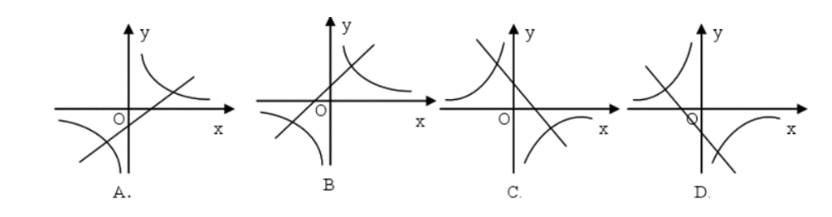
\includegraphics[scale=.7]{./images/0628_Graphs.png}
		\caption{$y = x + m$ and $y = \frac{m}{x}$.}
		\label{fig:0628_Graphs}
	\end{figure}
	\begin{solution}
		\textbf{B}.
		\begin{itemize}
			\item The straight line should be increasing, since the coefficient of $x$ is positive.
			      \textbf{C} and \textbf{D} are eliminated.
			\item If $m > 0$, the y-intercept of the straight line could not be negative.
			      \textbf{A} is eliminated, since the hyperbola in the same graph shows that $m>0$.
		\end{itemize}
	\end{solution}


	\question \qndate{29}{Jun} Given that points $A\left(-2,y_1\right)$, $B\left(-1,y_2\right)$,
	$C\left(1,y_3\right)$ are all on the graph of $y=-\oneover{x}$, arrange $y_1$,
	$y_2$ and $y_3$ in ascending order.
	\begin{solution}
		$y_3 < y_1 < y_2$.

		Subst. $x = -2$ into $y=-\oneover{x}$:
		\begin{align*}
			y_1 & = -\oneover{-2} \\
			    & = \oneover{2}
		\end{align*}

		Subst. $x=-1$ into $y=-\oneover{x}$:
		\begin{align*}
			y_2 & = -\oneover{-1} \\
			    & = 1
		\end{align*}

		Subst $x=1$ into $y=-\oneover{x}$:
		\begin{align*}
			y_3 & = -\oneover{1} \\
			    & = -1
		\end{align*}
	\end{solution}


	\question \qndate{30}{Jun} Given that points $\left(x_1,y_1\right)$, $\left(x_2,y_2\right)$
	and $\left(x_3,y_3\right)$ are all on the graph of $y=\frac{3}{x}$, also
	$x_1<x_2<0<x_3$, arrange $y_1$, $y_2$ and $y_3$ in ascending order.
	\begin{solution}
		$y_2<y_1<y_3$.
		\begin{itemize}
			\item $y_3 > 0$ since $x_3 > 0$. Hence, $y_3$ is the greatest.
			\item $0 > x_2 > x_1$, hence $y_2 < y_1 < 0$.
		\end{itemize}
	\end{solution}
\end{questions}
\end{document}
